\chapter{Einleitung}

\section{Problemstellung}
Sichtbarkeitsgraphen sind Graphen, die alle Knotenpaare miteinander verbinden, die sich \emph{sehen} können, auf deren \emph{Luftlinie} sich also keine \emph{Hindernisse} befinden.
Aus einer Küstenlinie kann ein Sichtbarkeitsgraph erstellt werden, indem die Knoten auf der Küstenlinie mit allen Knoten verbunden werden, deren Luftlinie keine Küste kreuzt.
\autoref{fig:thessaloniki-visibility} zeigt einen Ausschnitt eines solchen Sichtbarkeitsgraphen.
Zu sehen ist der Hafen der griechischen Stadt Thessaloniki.

Das Finden von kürzesten Pfaden ist in solchen Graphen rechenintensiver als etwa auf Straßengraphen mit vergleichbarer Knotenanzahl, da sie unter anderem einen höheren durchschnittlichen Knotengrad und keine inhärente hierarchische Struktur besitzen.
Zwar gibt es Möglichkeiten, den Graphen zu verändern, und schneller Pfade zwischen Knoten zu berechnen, etwa durch Triangulierung oder Rasterisierung, jedoch sind diese Pfade nicht mehr garantiert optimal.

Im Folgenden wird untersucht, inwiefern sich zwei Techniken zum schnellen Finden von kürzesten Pfaden und kürzesten Pfad-Distanzen (\emph{Contraction Hierarchies} und \emph{Hierarchical Hub Labeling}) auf diese Graphen anwenden lassen.

\begin{figure}[ht]%
    \centering
    \subfloat[\centering aegaeis-visibility]{{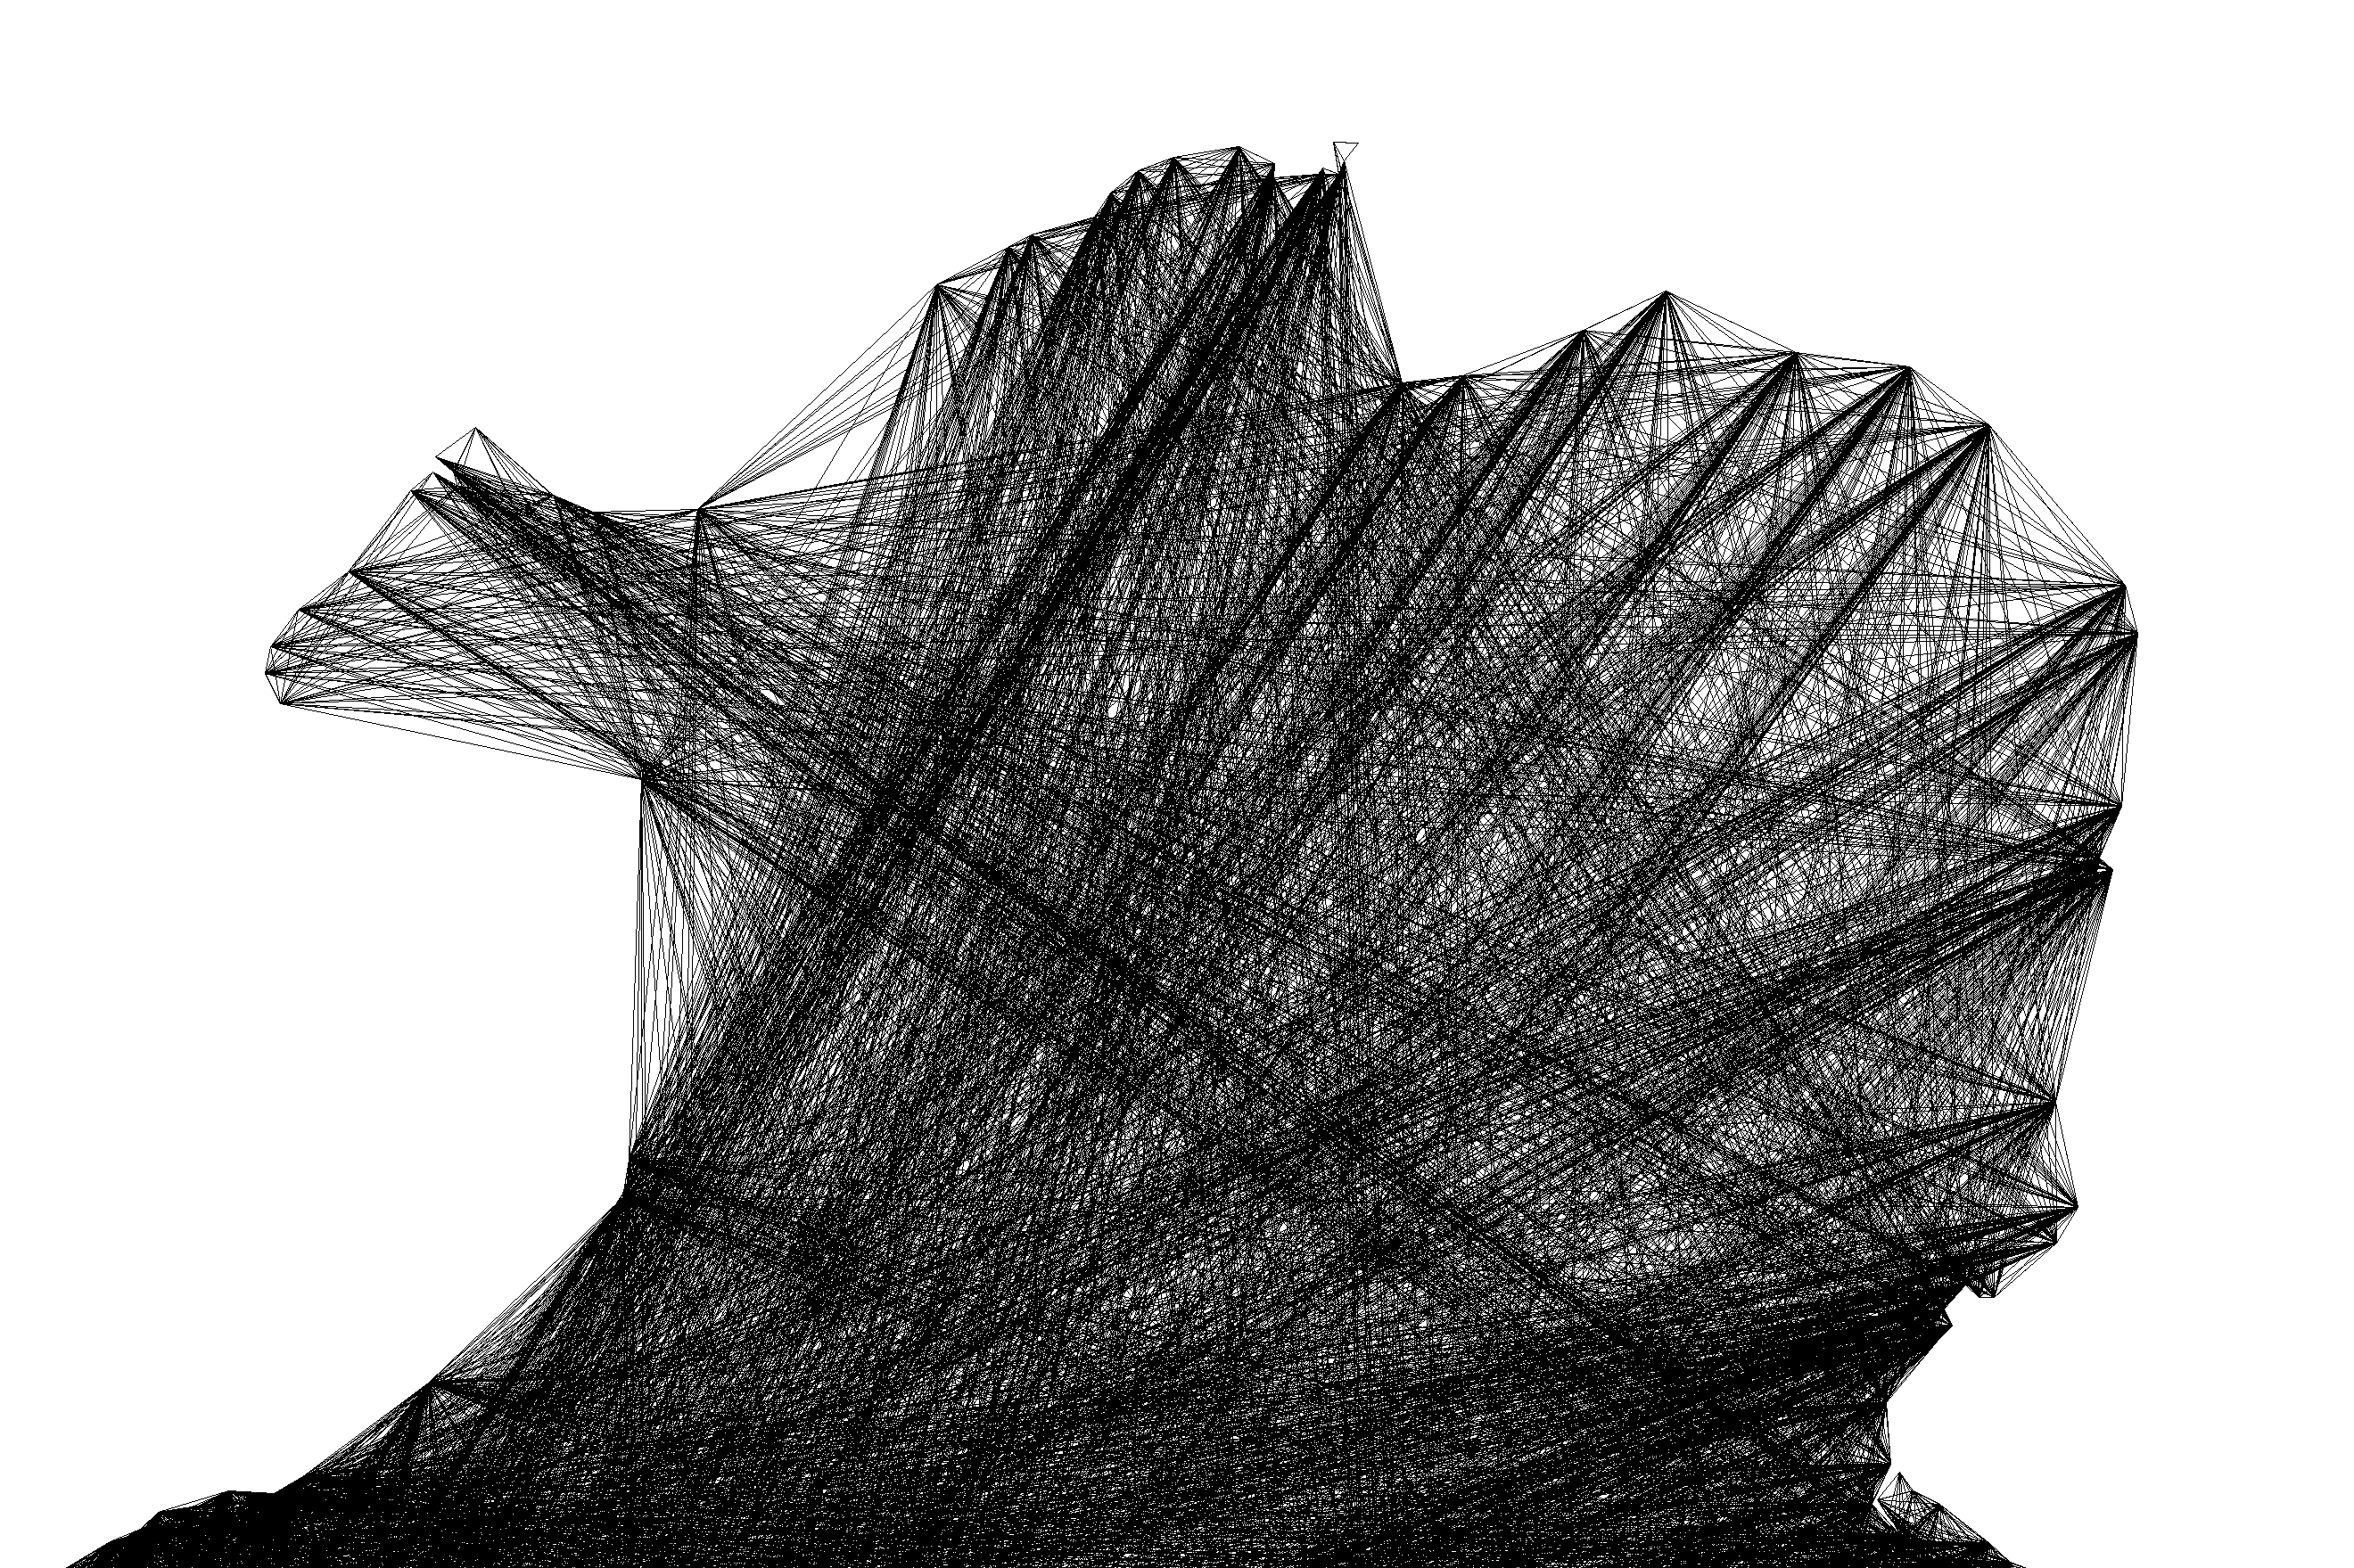
\includegraphics[width=.5\linewidth]{img/thessaloniki-visibility.png}}}%
    \caption{Sichtbarkeitsgraph des Hafens von Thessaloniki}%
    \label{fig:thessaloniki-visibility}%
\end{figure}

\section{Bearbeitete Graphen}

Der Fokus dieser Arbeit liegt auf drei Sichtbarkeitgraphen, welche jeweils einen Ausschnitt des Globus beinhalten.
Für jeden dieser drei Graphen existiert zusätzlich eine Triangulierung, deren kürzeste Pfade eine untere Schranke zu Sichtbarkeitgraphen darstellt
\autoref{table:input_graphs} listet die Graphen auf.
Die Graphen mit dem Präfix \emph{aegaeis} beinhalten das Ägäische Meer, mit \emph{medi} das Mittelmeer und mit \emph{pata} die Chilenische Fjorde.
Graphen mit dem Postfix \emph{visibility} sind Sichtbarkeitsgraphen, mit \emph{graph} Triangulierungen.
Die bearbeiteten Graphen sind ungerichtet, werden im folgenden jedoch als gerichtet betrachtet.
Insbesondere ist die in \autoref{table:input_graphs} aufgelistete Anzahl an Kanten gerichtetet zu interpretieren,
die ungerichtete Kante $\{a, b\}$ wird also doppelt gezählt als $(a, b)$ und $(b, a)$.

\begin{table}[ht]
    \centering
    \begin{tabular}{
            l % Graph
            S[table-format = 7.0] % Zeit
            S[table-format = 9.0] % Zeit
            S[table-format = 4.1] % Zeit
        }
        \toprule
        {Graph}            & {\# Knoten} & {\# Kanten} & {$\varnothing$ Grad} \\ \midrule
        aegaeis-graph      & 524881      & 2795322     & 5.32562999994        \\
        aegaeis-visibility & 201040      & 310231834   & 1543.13486868        \\
        medi-graph         & 795606      & 4223566     & 5.30861506826        \\
        medi-visibility    & 310114      & 730772544   & 2356.46421638        \\
        pata-graph         & 2240339     & 11632900    & 5.1924731034         \\
        pata-visibility    & 1002171     & 315653758   & 314.969958221        \\ \bottomrule
    \end{tabular}
    \caption{Bearbeite Graphen}
    \label{table:input_graphs}
\end{table}

\subsection{Triangulierung}

Die Triangulierung wird on \cite{funkescalable} erklärt.
Ein Beispiel solch einer Triangulierung ist in \autoref{fig:thessaloniki_comparison} gegeben.

\todo{Daniel nach Details fragen, wie die Triangulation zustande gekommen ist.}

Erst Triangulierung. Wenn Dreiecke sehr schmal sind, dann ersetzen durch Subdreiecke.

Die Knoten eines triangulierten Graphen $G_g$ bilden eine Obermenge zur Menge der Knoten des dazugehörigen Sichtbarkeitsgraphen $G_v$.
Die Triangulation darf den kürzesten Pfad Abstand zweier Knoten $a, b$ nicht verkleinern, aber vergrößern.


\begin{figure}[ht]%
    \centering
    \subfloat[\centering aegaeis-graph]{{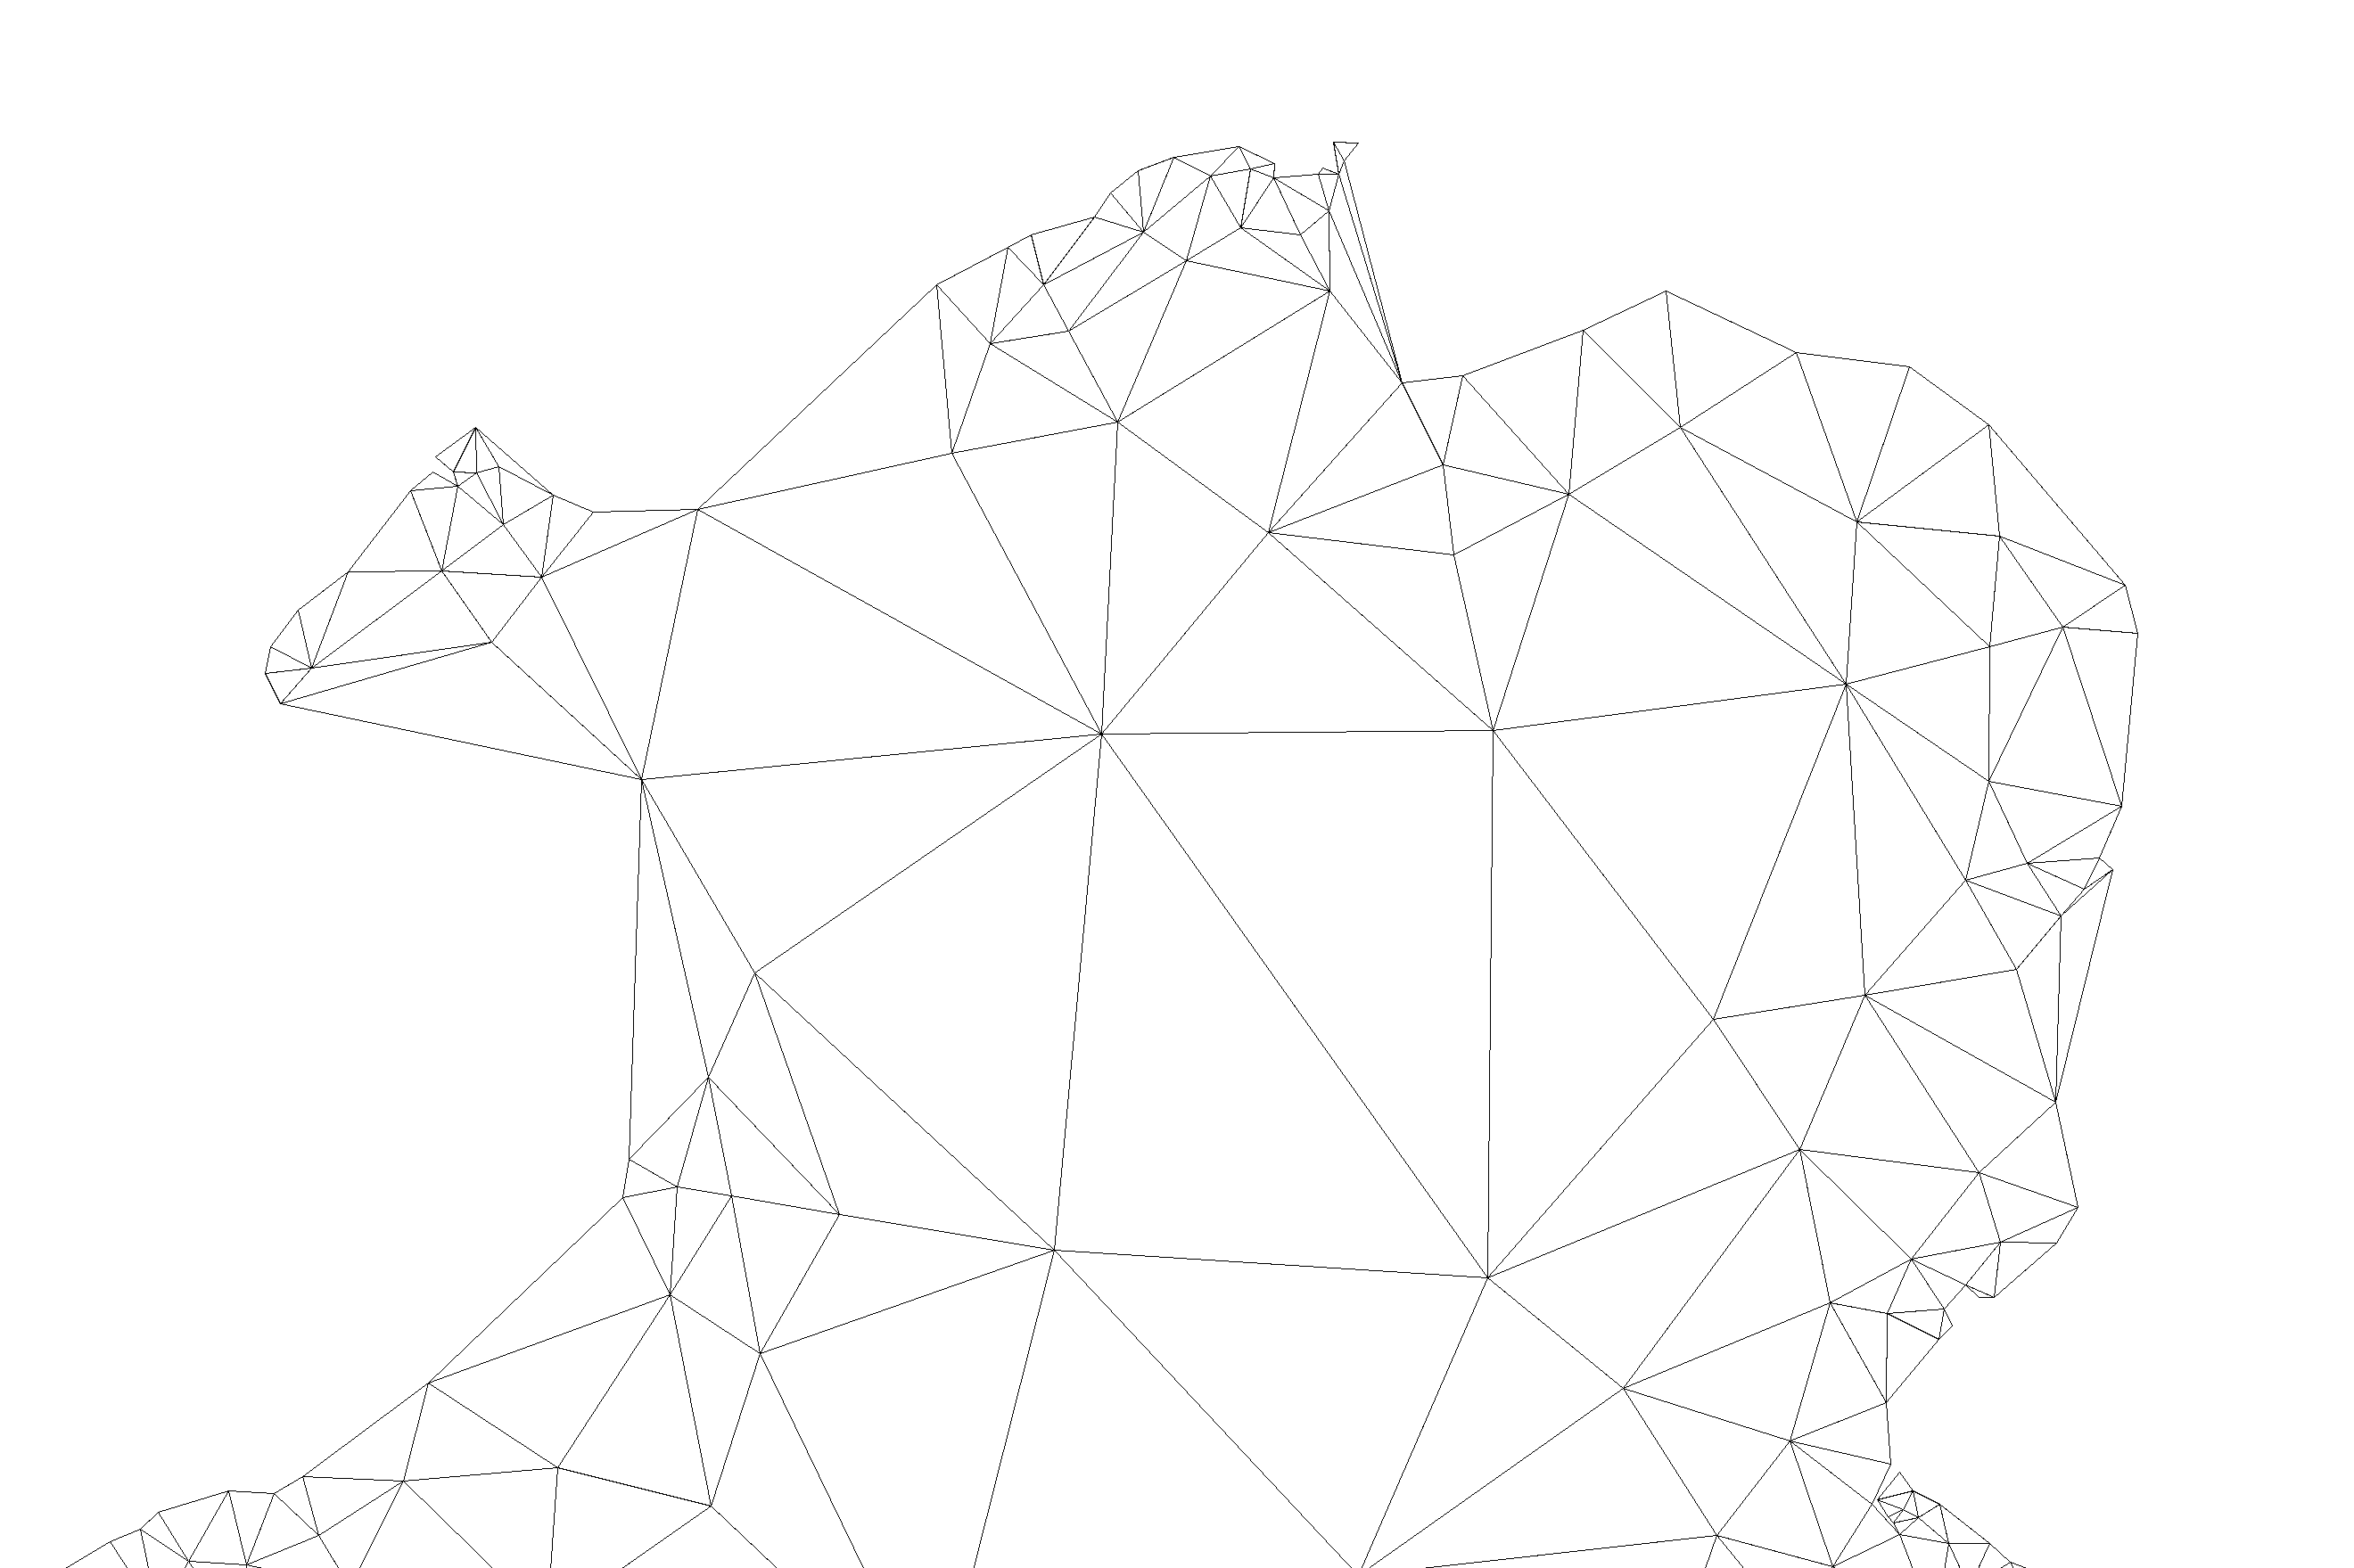
\includegraphics[width=.5\linewidth - 0.25cm]{img/thessaloniki-graph.png} }}%
    %\qquad
    \subfloat[\centering aegaeis-visibility]{{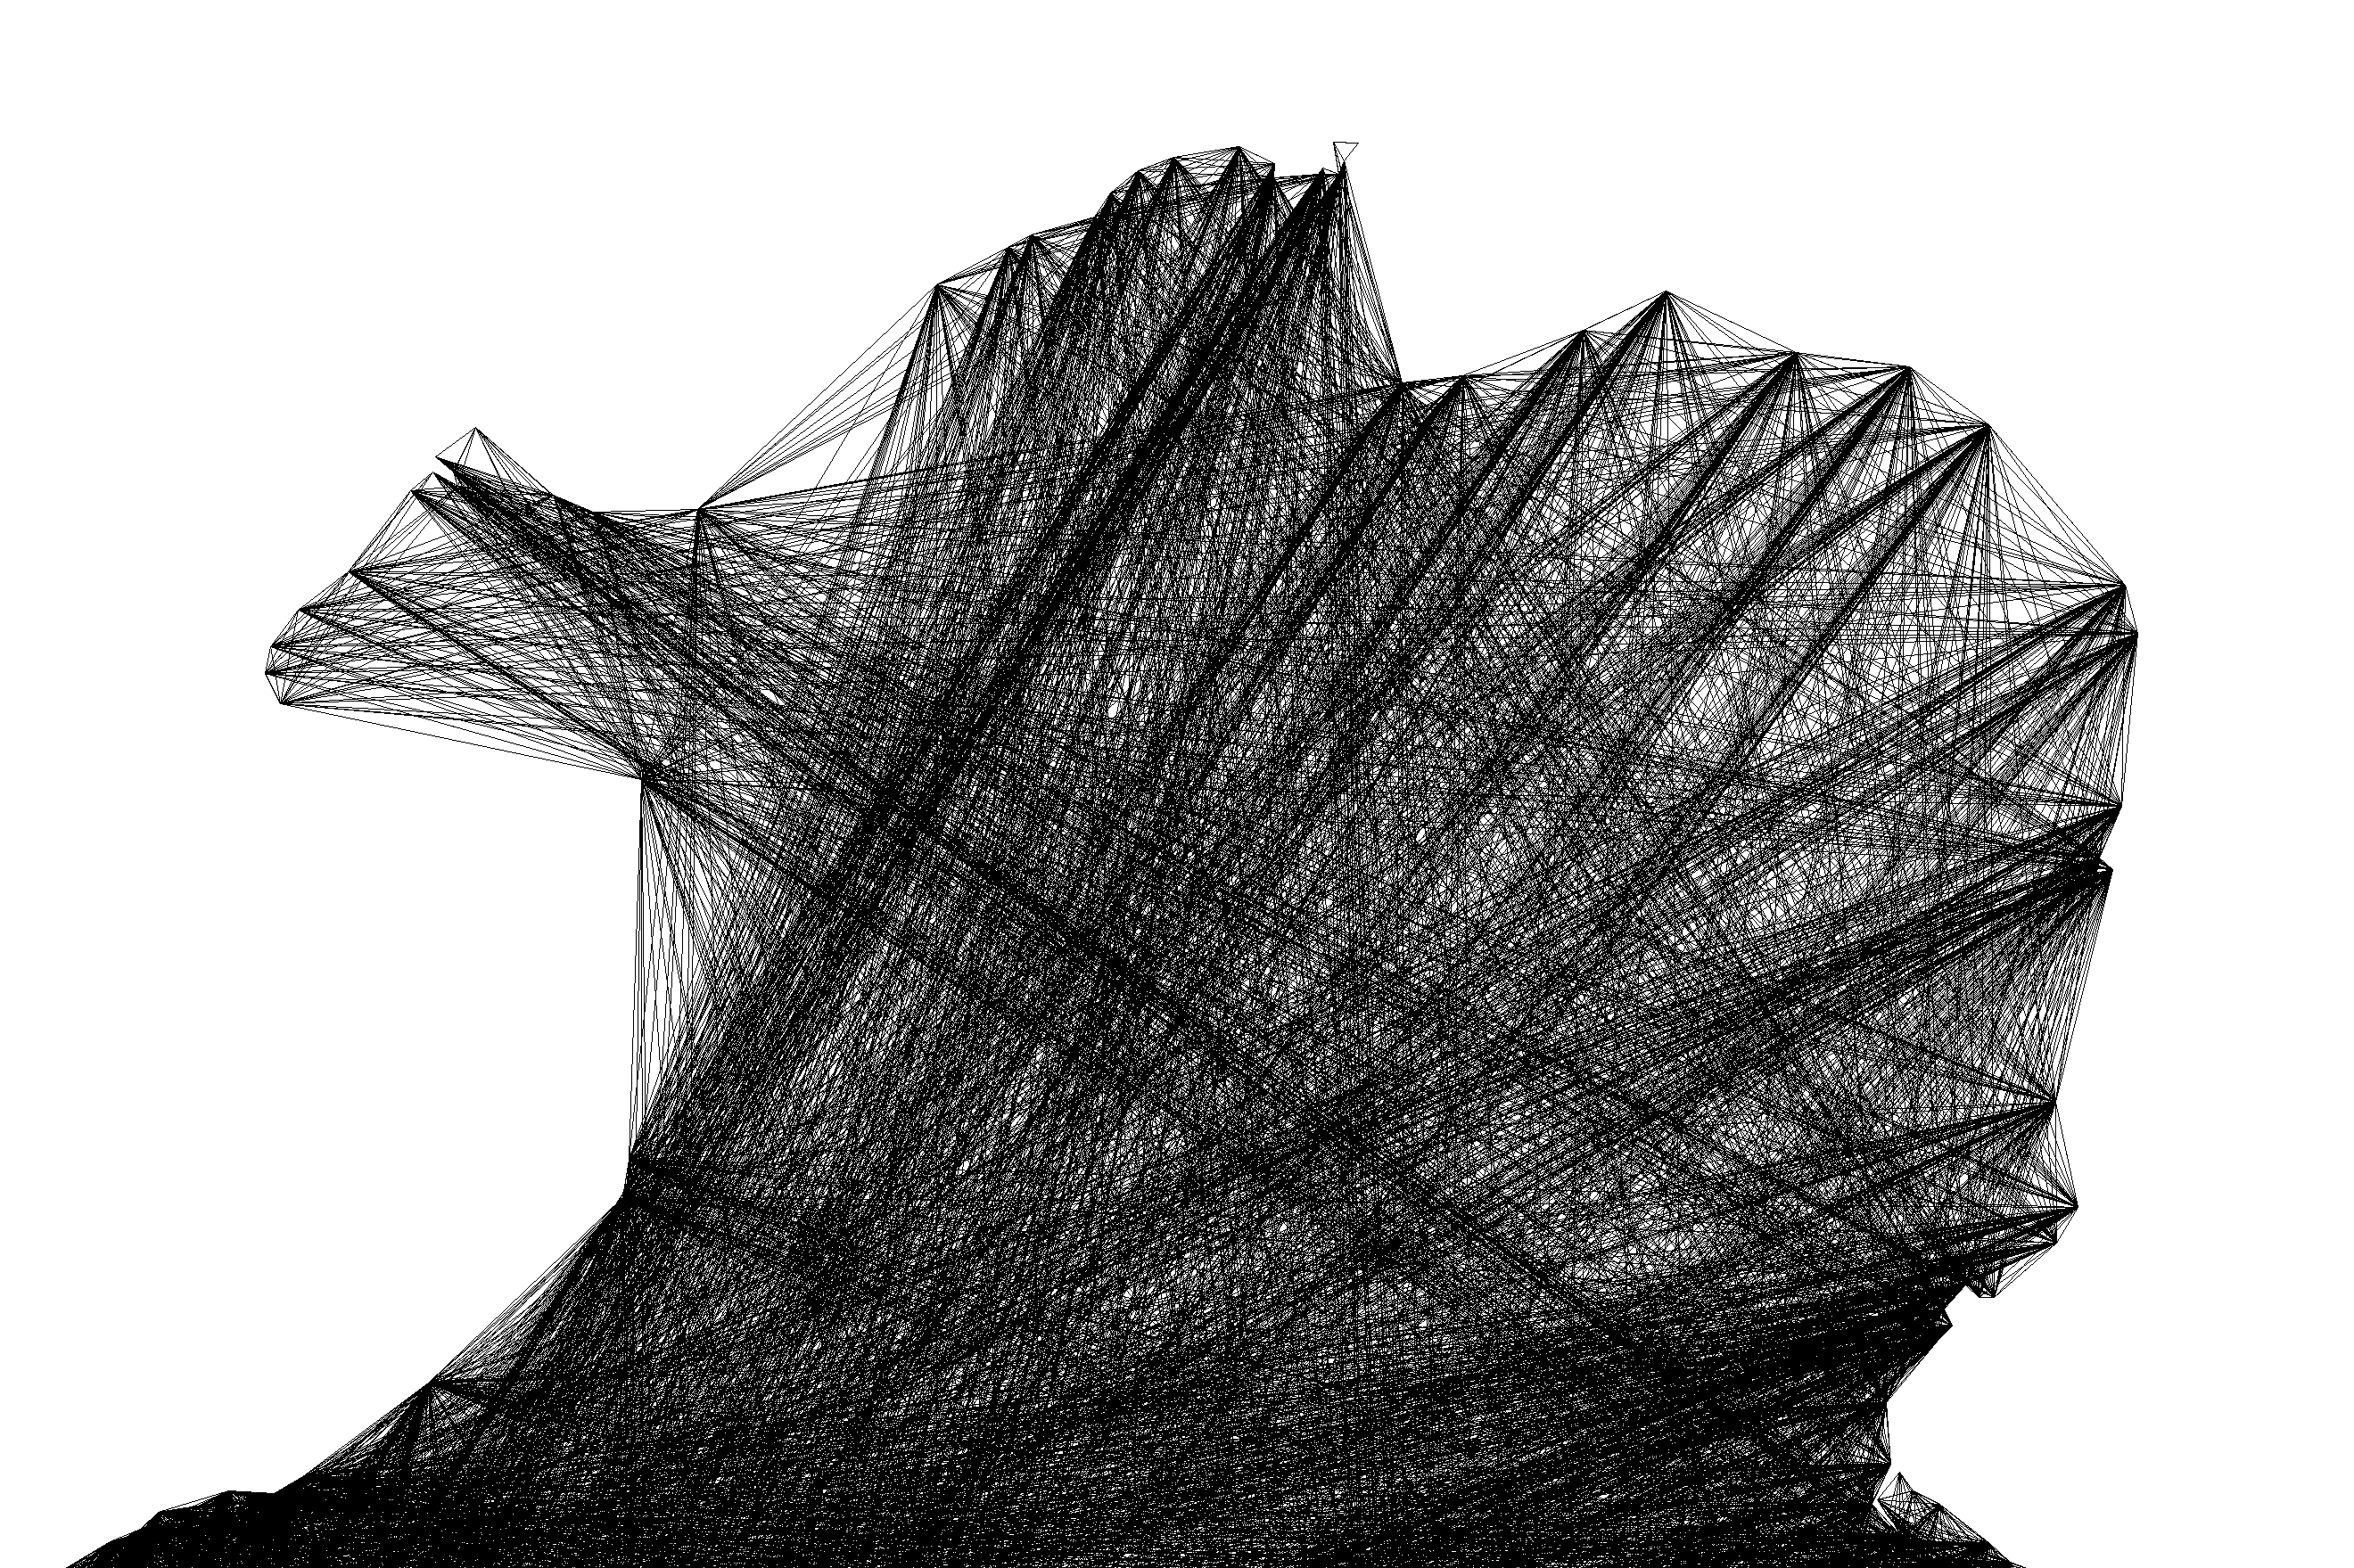
\includegraphics[width=.5\linewidth - 0.25cm]{img/thessaloniki-visibility.png} }}%
    \caption{Hafen von Thessaloniki}%
    \label{fig:thessaloniki_comparison}%
\end{figure}

\section{Speedup-Techniken}

Die betrachteten Speedup-Techniken zum Finden kürzester Pfade benötigen eine Phase der Vorbehandlung (\emph{preprocessing}), damit danach kürzeste Pfad Anfragen (\emph{queries}) schneller beantwortet werden können.
Die für das Preprocessing benutzte Rechenzeit und der Memory-Overhead sollte dabei in einem sinnvollen Verhältnis zum Speedup und der Anzahl der Queries stehen.
Ist der Speedup besonders hoch, so lohnt es sich mehr in das Preprocessing zu investieren.

\todo{Speedup Techniken auflisten}